\chapter{Revisão da Literatura}\label{arte}


\section{Introdução}\label{arte:intro}

Nesse capítulo, foi realizada uma revisão teórica e de pesquisas contemplando três campos, a saber: 
  \begin{itemize}
    \item O primeiro sobre o processo de aplicação da Mineração de Dados e Mineração em textos;
    \item O segundo relacionado às tecnologias mineração de dados relacionados à pesquisa em lide;
    \item Finalmente o último campo de pesquisa relacionado às tecnologias de mapeamento através de sistemas de posicionamento global 
    aplicados ao sistema rodoviário.
  \end{itemize}


  
\section{CRISP-DM}

O ``CRoss Indrustry Standard Process for Data Mining'' -- CRISP-DM é um processo para mineração de dados que descreve como especialistas 
nesse campo aplicam as técnicas de mineração para obter os melhores resultados \cite{Crisp2000}.
O CRISP-DM é um processo recursivo, onde cada etapa deve ser revista até quando o modelo apresentar os resultados satisfatórios, preliminarmente definidos.
O Analista de Dados ou o Cientista de Dados é o profissional que acompanha e executa o processo.

O CRISP-DM foi concebido, desenvolvido e refinado através de ``workshops'' entre 1996 e 1999 \cite{Crisp2000}, por três entidades empresariais europeias que 
formavam um consórcio, tendo com parceiros a Daimler-Chrysler AG (Alemanha), que estava, à época, à frente da maioria das organizações empresariais e comerciais 
na aplicação de mineração de dados em seus negócios; 
a SPSS Inc.(EUA), que provê serviços baseados em mineração de dados desde 1990, tendo lançado o primeiro workbench de mineração 
de dados comerciais o Clementine®; 
e a NCR Systems Engineering Copenhagen (EUA e Dinamarca), com o Teradata®, uma Datawarehouse que estabelecia equipes de consultores especialistas em mineração 
de dados para atender a seus clientes. Hoje mais de 300 empresas contribuem para o modelo de processo CRISP-DM.

\subsection{Contexto de aplicação do CRISP -- DM}

O contexto da aplicação do CRISP-DM \cite{Crisp2000} é guiado desde o nível mais genérico até o nível mais 
especializado, sendo normalmente explicado em quatro dimensões:

\begin{itemize}
 \item O domínio da aplicação -- a área específica que o projeto de mineração de dados acontece;
 \item O tipo de problema -- descreve as classes específicas do objetivo do projeto de mineração de dados;
 \item Os aspectos técnicos -- cobrem as questões específicas como os desafios usualmente encontrados durante o processo de mineração de dados; 
 \item As ferramentas e técnicas -- dimensão específica que cada ferramenta/técnica de mineração de dados é aplicada durante o projeto.
\end{itemize}

A tabela abaixo sumariza e exemplifica essas dimensões no contexto de aplicação do CRISP-DM.

\begin{table}[!ht]

\caption{Mineração de dados -- contexto de aplicação \cite{Crisp2000}}
\vspace{1mm}
\centering
\begin{tabular}{c|c|c|c|c}
\textbf{Dimensão} & \textbf{Domínio da} & \textbf{Tipo de } & \textbf{Aspecto } & \textbf{Ferramentas } \\
		  & \textbf{aplicação}  & \textbf{Problema} & \textbf{técnico}  & \textbf{e Técnicas}   \\ \hline
\textbf{Exemplo}  & Modelo de           & Descrição e       & Dados             & Clementine  \\
                  & resposta            & sumarização       & faltantes         &             \\ \hline
      --- 	  & Predição            & Segmentação       & \textit{Outlies}  & MineSet     \\
         	  & agitada             &                   &                   &             \\ \hline
      ---         & ---                 & Descrição do      & ---               & Árvore de   \\
                  &                     & conceito          &                   & decisão     \\ \hline
      ---         & ---                 & Classificação     & ---               & ---         \\ \hline
      ---         & ---                 & Predição          & ---               & ---         \\ \hline
      ---         & ---                 & Análise de        & ---               & ---         \\
                  &                     & dependências      &                   & \\            
\\
\end{tabular}
\tiny Fonte: CRISP-DM -- 1.0
\end{table}


A aplicação das técnicas de mineração de dados identifica padrões ocultos nos dados, inacessíveis pelas técnicas tradicionais,
como por exemplo, consultas em banco de dados, técnicas estatísticas, dentre outras. Além disso, possibilita analisar um grande número de 
variáveis simultaneamente, o que não acontece com o cérebro humano \cite{possas1998data}, bem como, com outras técnicas. 
A análise desse processo permite extrair novos conhecimentos a partir dos dados, que é tratado na literatura como 
KDD -- Knowledge Discovery Database \cite{FayyadUeoutros}. Fayyad destaca a natureza interdisciplinar do KDD que contempla a intersecção 
de campos de pesquisa tais como Aprendizagem de Máquina (Machine Learning), Reconhecimento de Padrões, I.A., estatística, computação de alto 
desempenho e outros, propõe que o objetivo principal é extrair um conhecimento de alto nível a partir de dados de baixo nível num contexto de 
grandes bases de dados.
O CRISP-DM, por sua vez, engloba todos esses elementos como pode ser visto na figura a seguir:

\begin{figure}[!ht]
\centering
\caption{Domínio das técnicas aplicadas a mineração de dados}
\vspace{1mm}
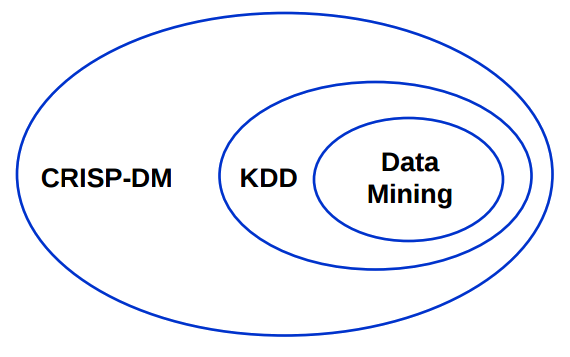
\includegraphics[width=90mm, height=40mm]{Figuras/BigData/RelacaoCrispKddDm.png}\\
\tiny Fonte: Neurotech -- 2012
\end{figure}

\pagebreak

\subsection{Ciclo de vida do CRISP--DM}

O modelo de processo CRISP--DM provê seis fases para um projeto de mineração de dados, sendo assim determina-se um ciclo de vida 
compreendido para cada uma dessas fases:

A figura a seguir ilustra as fases do ciclo:

\begin{figure}[!ht]
\centering
\caption{O padrão CRISP-DM \cite{Crisp2000}}
\vspace{1mm}
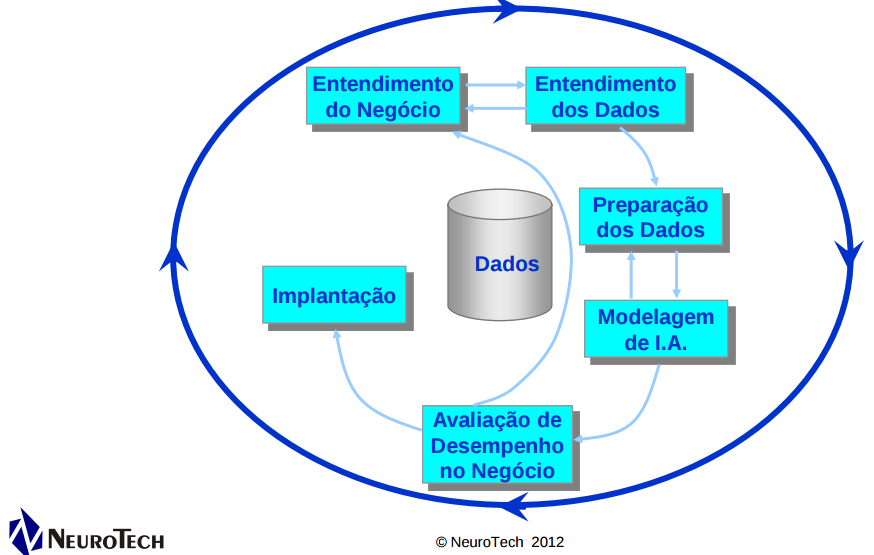
\includegraphics[width=100mm, height=75mm]{Figuras/BigData/CrispDM.png}\\
\tiny Fonte: CRISP-DM 1.0
\end{figure}

A primeira fase, conhecida como \textbf{Entendimento do negócio}, ou ``fase de entendimento dos objetivos e dos requerimentos sob a 
perspectiva do negócio'' (CHAPMAN; KERBER; WIRTH et al, 2000, p.{10}) é uma fase crucial da mineração,  um especialista (ou muitos) deve ser consultado. 
O analista de dados e o analista do negócio traçam os objetivos da mineração sob a perspectiva do cliente. Questionamentos incorretos 
ou negligência nesta fase podem acarretar esforços excessivos no processo como um todo a experiência de um profissional da área 
é condição ``sine qua non'' nessa fase. Portanto avaliar o negócio, avaliar a situação sob o ponto de vista dos riscos de não conclusão 
do processo, determinar os objetivos e traçar um plano para execução. Essas etapas são delineadas nas figuras que se seguem.

\begin{figure}[!ht]
\centering
\caption{Entendimento do negócio}
\vspace{1mm}
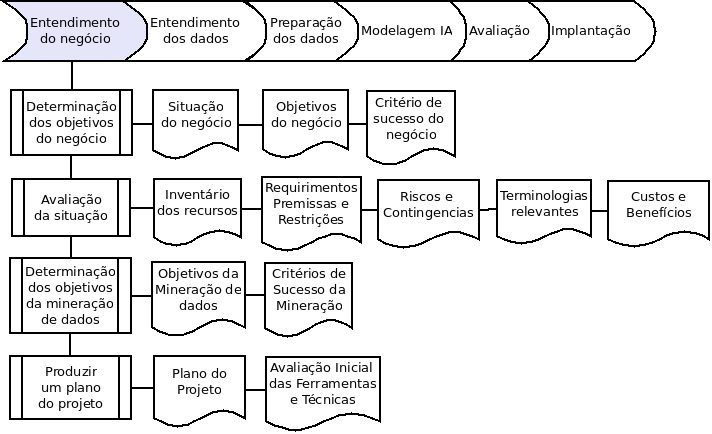
\includegraphics[width=120mm, height=75mm]{Figuras/Cronograma/Entendimento.png}\\
\tiny Fonte: CRISP-DM 1.0
\end{figure}

\pagebreak

\vspace{0.5cm}

Em seguida, o analista de dados passa à segunda fase, \textbf{Entendimento dos dados}. Nessa fase o analista ``olha'' para os dados com a acurácia de um especialista, 
procurando identificar qualidade nos dados. Dados ausentes -- ``missing data'' -- são comuns em bases de dados não estruturadas, configurando-se como
um problema a ser considerado, pois seu tratamento pode consumir muito tempo do analista de dados. 

\begin{figure}[!ht]
\centering
\caption{Entendimento dos dados}
\vspace{1mm}
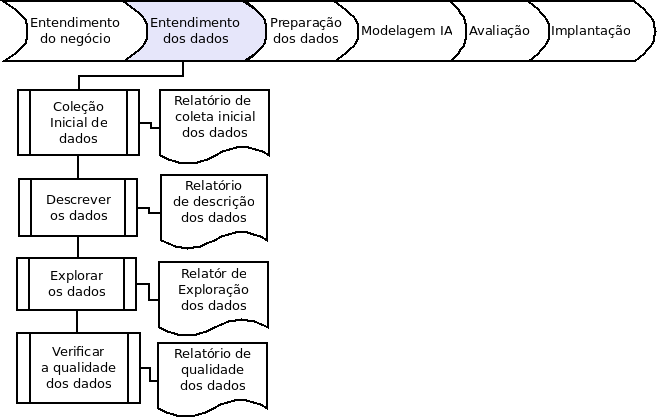
\includegraphics[width=120mm, height=75mm]{Figuras/Cronograma/EntendDados.png}\\
\tiny Fonte: CRISP-DM 1.0
\end{figure}

\vspace{0.5cm}

A terceira fase, \textbf{Preparação dos dados}, diz respeito à construção final do conjunto de dados. 
Preparar os dados significa criar e selecionar atributos, criar tabelas ou planilhas e registros dos dados.

\pagebreak

\begin{figure}[!ht]
\centering
\caption{Preparação dos dados}
\vspace{1mm}
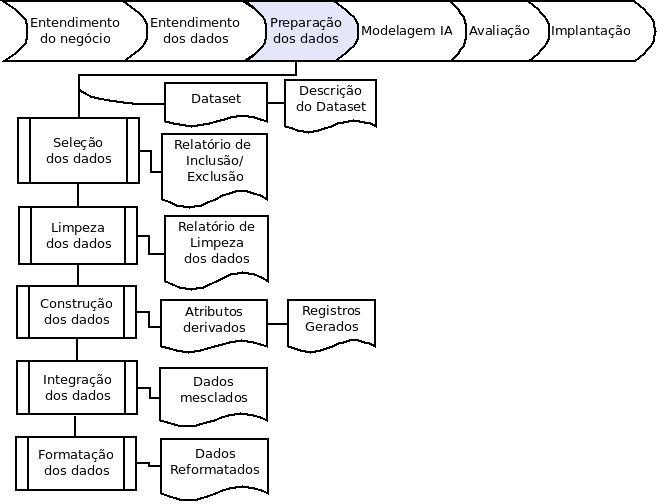
\includegraphics[width=120mm, height=90mm]{Figuras/Cronograma/PreparaDados.png}\\
\tiny Fonte: CRISP-DM 1.0
\end{figure}

\vspace{0.5cm}

Na quarta fase, \textbf{Modelagem de I.A.}, a tecnologia deve ser escolhida de forma criteriosa, baseada na experiência do analista de dados. 
Em sistemas de suporte à decisão, uma tecnologia inadequada pode levar a decisões imprecisas. É comum retornar às fases anteriores para adequar a técnica aos dados. 
Um modelo de regressão logística para problemas binários, redes neurais para problemas de classificação, e assim por diante.

\begin{figure}[!ht]
\centering
\caption{Modelagem IA}
\vspace{1mm}
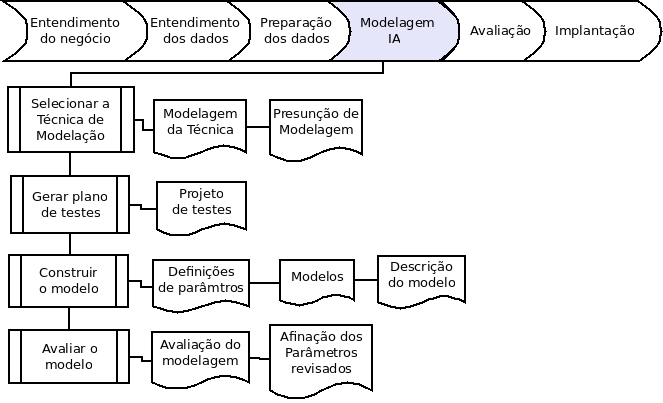
\includegraphics[width=120mm, height=79mm]{Figuras/Cronograma/Model_IA.png}\\
\tiny Fonte: CRISP-DM 1.0
\end{figure}

\vspace{0.5cm}

Na fase cinco, \textbf{Avaliação de desempenho}, um ou muitos modelos devem ter sido construídos e testados, 
de forma que seja possível atingir uma alta qualidade do ponto de vista da análise dos dados, ou seja, que o 
modelo proposto esteja de adequado aos objetivos do negócio. Para tal é preciso que antes do desenvolvimento final 
do modelo, os passos executados até então sejam avaliados e revistos.

\begin{figure}[!ht]
\centering
\caption{Avaliação do modelo}
\vspace{1mm}
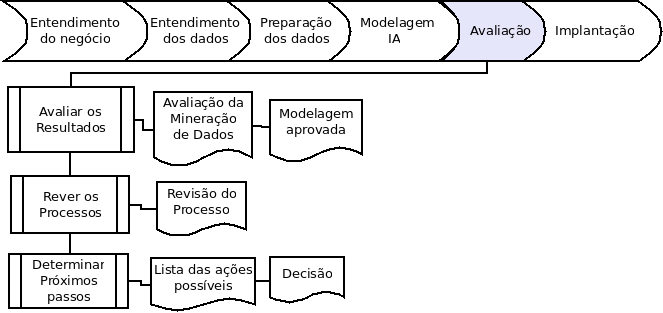
\includegraphics[width=120mm, height=65mm]{Figuras/Cronograma/Avaliacao.png}\\
\tiny Fonte: CRISP-DM 1.0
\end{figure}

%\pagebreak

A sexta e última fase, caracteriza-se pela conclusão do modelo. No entanto a criação do modelo não é o fim do processo.
O conhecimento adquirido precisa ser incrementado, organizado e apresentado de maneira que o cliente possa usá-lo.
É importante ressaltar que este ciclo poderá ser retomado até que o modelo esteja adequado às necessidades e especifidades do cliente.

\begin{figure}[!ht]
\centering
\caption{Implantação do modelo}
\vspace{1mm}
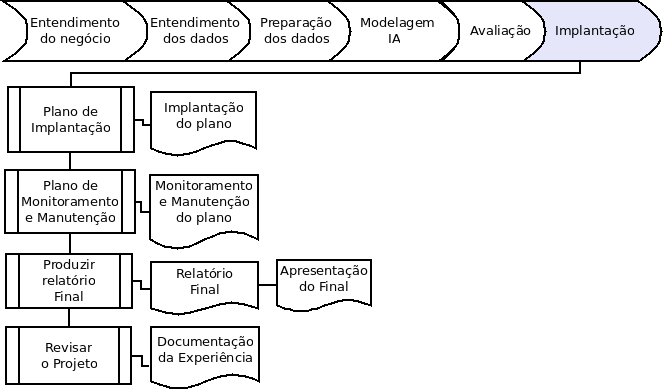
\includegraphics[width=120mm, height=75mm]{Figuras/Cronograma/Inplantacao.png}\\
\tiny Fonte: CRISP-DM 1.0
\end{figure}


\pagebreak

%\section{Além do KDD -- \textit{Domain-Driven for Data Mining}}


\pagebreak

\section{Mineração de dados}

No processo de extração do conhecimento (KDD), um dos importantes passos a ser considerado é a mineração de dados, que se caracteriza pela aplicação de algoritmos 
específicos para descoberta de padrões e/ou comportamentos em grandes bases de dados, também conhecido como repositórios de dados \cite{FayyadUeoutros}.

A mineração se distingue das técnicas estatísticas pelo fato de que  não trabalha com dados hipotéticos, mas se apoia nos próprios dados para extrair os padrões (CASTANHEIRA, 2008). 

FAYYAD (1996), destaca que é necessário distinguir claramente KDD e mineração de dados. Enquanto que é um processo, a mineração é um passo no interior desse processo. 
Todavia, esse passo é de considerável relevância para que se possa extrair conhecimento adequadamente. 
A aplicação “cega” dos métodos de mineração de dados, ainda segundo Fayyad (1996), pode conduzir à descoberta de dados sem significado e padrões inválidos. 

Existem vários tipos de dados e informações nesses repositórios que podem ser minerados, contudo esses dados, inicialmente são selecionados e agrupados, a seguir passam por 
uma fase de preprocessamento, que consiste em tratá-los de forma a prepará-los para a mineração. Essa fase é de 
fundamental importância na estruturação dos dados, uma vez que em grandes volumes de dados, também conhecido ``Datawarehouse'', podem existir inconsistências, faltas (missing data) ou 
duplicidade e erros de informações.

Nesse sentido, as técnicas de mineração de dados trabalham com dados estruturados, preenchidos em sua totalidade sem \textit{missing data}, para poder extrair informações relevantes.
Existem várias maneiras de se contornar os dados ausentes, como o preenchimento dos dados através de técnicas de inteligência artificial, da média dos valores; quando dados numéricos 
ou com a moda; quando os dados forem categóricos. Para cada tipo de dados existem técnicas apropriadas para serem aplicadas sobre eles, algumas mais sensíveis às problemáticas elencadas anteriormente
e outras mais robustas \cite{DataMining2}, que por sua vez estão associadas a classes de problemas que a mineração trata, a tabela 2.1 delineou o domínio.
Isso será tratado na seção Aprendizagem de Máquina (Machine Learning).
O caminho da extração dos dados até sua mineração e extração de conhecimento é longo.
Na figura a seguir temos a ilustração desse caminho:

\begin{figure}[!ht]
\centering
\caption{Fases da mineração de dados até extração do conhecimento}
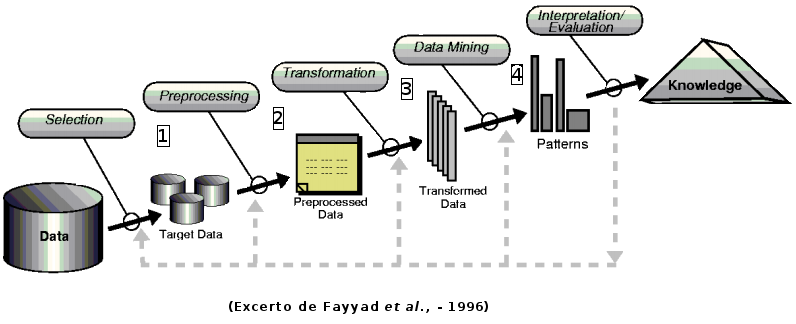
\includegraphics[width=135mm, height=65mm]{Figuras/BigData/FayyadSemFundo.png}
\end{figure}



A origem dos dados, os ``inputs'' estão representados na figura onde se lê ``Data'' este está repleto de \textit{missing data} e/ou dados inconsistentes, conhecidos como dados não estruturados. 
O balão onde se lê ``Selection'' representa a coleta das informações ou a seleção dos dados no \textit{Big Data}.
Em nossa pesquisa esses dados são provenientes das mais diversas fontes, tais como, redes sociais, câmaras de trânsito, informações de satélites meteorológicos e outras fontes.

Armazenar dados provenientes de redes sociais nessa etapa pode ser um grande problema, devido à sua extensão, porém os dados relevantes podem ser armazenados em ``Target Data'' 
com tecnologia apropriada, utilizando-se técnicas de ``Map'' e ``Reduce'' ou mineração de dados em textos para criar \textit{cluster} de informações e ler os fluxos de dados (stream data). 
Algumas técnicas de IA podem ser aplicadas nessa etapa como, [``Data Mininng Swarm Robotics'' através de Botnets \footnote{Botnet é citado no sentido da coleta de informações} ou ``Swarm Intelligence''. ]

No balão ``Preprocessing'' os dados não-estruturados são tratados, por exemplo, retirando os \textit{missing data}. 
Para estruturar as informações é preciso utilizar técnicas linguísticas, uma vez que existe lógica entre eles \cite{Aranha2006}.
Esses dados normalmente são coletados por técnicas de Mineração de Textos, também conhecidas como Mineração de Dados em Textos, técnicas de IA como ``Machine Learning'' 
têm sido muito utlizadas. Em ``Transformation'' os dados foram em estruturados, podendo ser armazenados em Bancos de Dados, conhecidos como Datawarehouse, por exemplo o Hive. 

O processo de Mineração dos dados começa no balão ``Data Mining'', onde são aplicadas as técnicas de IA conhecidas como classificadores, para extração de padrões, tais como: 
``Decision Tree'' (Árvore de decisão), ``Artificial Neural Network'' (Redes neurais artificiais), ``Logistic Regression'' (Regressão Logística) e ``Deep Learning''.
Algumas técnicas de mineração de dados são fortemente influenciadas pelas informações na entrada (input), como as Árvores de decisão \cite{DecisionTree}. 
As Redes Neurais, dependendo da quantidade de variáveis de entrada, paderão ter milhares de neurônios na camada intermediária, o que inviabilizaria essa metaheurística 
\footnote{Metaheurística são heurísticas aplicadas em problemas onde os custos computacionais não são tratáveis em tempo polionomial, devido às explosões combinatórias geradas
pelo grande número de tentativas. Metaheurísticas bioinspiradas metaforizam o comportamento de animais sociais, tais como formigas, pássaros, peixes e outros}.

Todas essas etapas descritas na figura são recorrentes, como indicam as setas pontilhadas que retornam aos passos anteriores.
Utilizar técnicas de mineração de dados, além de extrair dados, extrai conhecimento, com isso pode-se predizer os resultados futuros na saída do modelo, 
quando determinados dados ocorrem na entrada \cite{Amin2015a}, essa técnica de extração de conhecimento chama-se \textit{Knowledge Discovery Databases} (KDD).
O KDD utiliza métodos de Aprendizagem de Máquina para efetuar essa extração.



\pagebreak


\section{Tipos de Aprendizagem}

\color{blue} {Fulano classifica aprendizado supervisionado como .... }

\color{red} {Beltrano classifica aprendizagem não supervisionada como ...}

\color{black}

Para ``aprender'' sobre uma determinada função \textit{f} definimos uma amostra em um conjunto de treinamento $X = {x_{1}, x_{2}, ...x_{n}}$.







As técnicas algorítmicas apresentadas nas seções subsequentes são parte da grande família de algorítimos que compõem 
o aprendizado de máquina aplicado a mineração de dados.

A descoberta de conhecimento através da aplicação das técnicas de mineração de dados podem ser agrupadas de acordo com suas funcionalidades \cite{DataMining2}, 
essas funcionalidades tem como característica principal a maneira como são descobertos os padrões no dados, elas podem estar 
em uma das duas categorias: tarefas descritivas ou tarefas preditivas. As tarefas mineração descritivas preocupam-se nas características 
dos dados no conjunto de dados; o ``data set''. As tarefas de mineração preditivas induzem regras nos dados correntes para produzirem 
predições \cite{DataMining2}. A seção seguinte analisa as tarefas preditivas.




\subsection{Aprendizagem de Máquina}\label{arte:palavraChave:Machine}


Aprendizagem de Máquina ou ``Machine Learning'' são métodos para analisar dados de forma automatizada e interativa.
Segundo Shalev-Shwartz \& Ben-David \cite{Ben-David2014} em seu livro ``Understandig Machine Learning: From Theory to Algorithms'' 
o termo Aprendizagem de Máquina refere-se à detecção automatizada de Padrões de dados.

Para Nilsson \cite{Nilsson2005} o aprendizado ocorre quando uma máquina modifica sua estrutura interna, programa ou dados 
(baseados nos inputs ou em uma resposta para informação externa) de tal maneira que melhora o desempenho futuro. Por exemplo quando uma 
máquina de reconhecimento da fala \textbf{melhora} após ``ouvir'' várias amostras de fala humanas e que nós sentimos que pronta, neste caso
podemos dizer que a máquina aprendeu. 

Sistemas que executam tarefas de inteligência artificial tais como Reconhecimento de Padrões, Diagnóstico, Controle de Robôs, Predição e 
outros precisam ser modificados para executarem ``Machine Learning'' \cite{Nilsson2005}.


\subsection{Aprendizagem Bayesina}



\subsection{Onde e o que aprender}

Historicamente os tipos de aprendizagem computacional estão relacionados em ``o que'' há para ser aprendido \cite{Nilsson2005}. 
Primeiramente para escolher o que aprender definiremos de ``onde'' ou sobre quais dados se aprender.
Fornecemos um conjunto de treinamento para depois testar o conhecimento aprendido em um conjunto de teste.


\section{Classificação e Regressão para análise preditivas}

Classificação é um processo para encontrar um modelo que descreve e distingue classes de dados. 
Esse modelo tem como base de análise um conjunto de treinamento (i.e. objetos de dados para os quais 
serão encontrados rótulos que os classifiquem). 
Esse modelo é usado para predizer quais rótulos de classes terão os objetos desconhecidos.
O modelo pode ser representado por regras de classificação do tipo ``IF - THEN'', por árvores de decisão, redes neurais e outros. 
Regras de classificação se distinguem de regras de indução da seguinte forma:
\begin{itemize}
 \item Uma regra de classificação poderia ser: $if$ L $them$ class = $C_{1}$ ou $if$ L $them$  $C_{1}$
 \item Uma regra de indução seria: $ if$ L $them$ R que por sua vez produz novas regras 
\end{itemize}

As árvores de decisão são estruturas como fluxogramas, possuem nós e ramificações, 
cada nó é um teste no valor do atributo como:
\singlespace

\begin{figure}[ht] \unitlength= 1mm \thicklines
 \centering{
    \begin{picture}(100,6)
      \put(0,0){\framebox(115,6)} \put(3,2){$age(X,``youth")$ AND $income(X,``high")  \to classe (X,``A")$}
      \put(0,-7){\framebox(113,6)} \put(3,-5){$age(X,``youth")$ AND $income(X,``low") \to classe (X,``B")$}
      \put(0,-14){\framebox(85,6)} \put(3,-12){$age(X,``middle-aged")$  $\to classe (X,``B")$}
      \put(0,-21){\framebox(70,6)} \put(3,-19){$age(X,``senior")$  $ \to classe (X,``B")$}
      \end{picture}
   }
\end{figure}

\vspace{20mm}
  
A seguir, a árvore de decisão que explicita se um cliente, de acordo com sua idade terá determinada classe:
\begin{figure}[!ht]
\centering
\caption{Árvore de decisão}
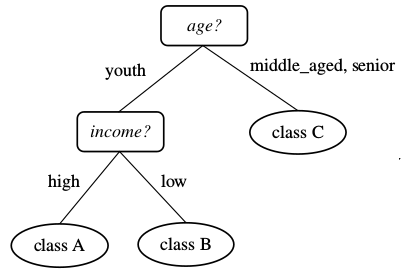
\includegraphics[width=60mm, height=45mm]{Figuras/BigData/arvorejovem.png}\\
\tiny Fonte: Han, J. and Kamber, M. 
\end{figure}  

A figura a seguir representa uma rede neural com as mesmas características da árvore de decisão anterior:
\begin{figure}[!ht]
\centering
\caption{Rede Neural}
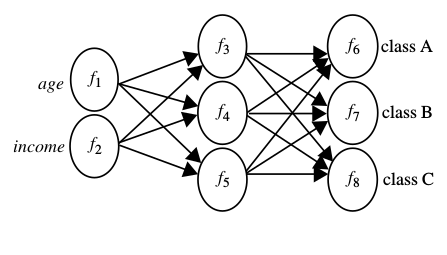
\includegraphics[width=85mm, height=38mm]{Figuras/BigData/redeneural.png}\\
\tiny Fonte: Han, J. and Kamber, M. 
\end{figure}  

As árvores de decisão produzem regras de indução, são algoritmos rápidos, contudo dados impuros podem comprometer o desempenho desse algoritmo. 
A fase de extração dos dados do é fortemente influenciáveis pelas variáveis escolhidas, \cite{DecisionTree} 
isso pode representar o desafio maior para implementar esta técnica. 

Outro problema que pode ser encontrado em algoritmos de aprendizagem é o ``overfitting'' ou superadaptação aos modelos.
Segundo RUSSEL E NORVIG (2004)  \footnote{Foi observado que redes neurais muito grandes \textit{generalizam} bem, 
\textit{desde que os pesos sejam mantidos pequenos}. Essa restrição mantém os valores de ativação na região 
\textit{linear} da função sigmóide g(x) onde x é próximo de zero. Por sua vez isso faz com que a rede se comporte 
como uma função linear, com um número muito menor de parâmetros.} o ``overfitting'' ocorre quando o número atributos é grande.



\pagebreak

\section{Árvore de Decisão}

Han e Kamber \cite{DataMining} definem indução por árvore de decisão como a aprendizagem de árvore de decisão a partir de classes rotuladas nas tuplas de treinamento. 
A estrutura da árvore de decisão é semelhante a um fluxograma, onde cada nó interno (não-folha) indica um teste de atributo, cada ramo representa o resultado de um teste e 
cada nó da folha possui um rótulo de classe. O nó de nível mais superior é chamado de nó-raiz.


Para Ian e Frank \cite{MachineLearning}, as árvores de decisão podem ser representadas por uma abordagem ``dividir para conquistar'' para resolução de problemas de 
aprendizagem, a partir de um conjunto de instâncias independentes. Os nós em uma árvore de decisão ``testam'' um atributo específico, comparando seu valor com uma constante.
No entanto, algumas árvores podem comparar dois atributos com outros ou utilizarem uma função para tal.
As árvores de decisão podem ser classificadas em dois tipos: árvores de regressão (regression trees), que são utilizadas para estimar atributos numéricos, e árvores de 
classificação (classification trees), usadas para análise de variáveis categóricas.


\subsection{Tipos de Árvores de decisão}
O algorítimo \textit{C4.5} é considerado um exemplo clássico de método de indução de árvores de decisão. O \textit{C4.5} \cite{Learning2007} foi inspirado no algoritmo 
\textit{ID3} \cite{Learning1979}, que produz árvores de decisão a partir de uma abordagem recursiva de particionamento de um conjunto de dados, utilizando conceitos e medidas 
da Teoria da Informação \cite{TeoriaInf}.

As árvores de decisão têm uma característica peculiar, a saída do modelo de predição (o output), com regras se -- então é claramente perceptivel por analistas humanos.
Essa qualidade é utilizada para interpretar os resultados.


\section{Regressão}

\subsection{Tipos de regressão aplicadas a mineração de dados}

((( incluir e explicar ao menos 3 tipos )))

\subsection{Regressão Linear}

\subsection{Regressão Logística}
Regressão logística (linear, logística, ou outras) é uma técnica para analisar o relacionamento entre variáveis. No entanto, a regressão linear é utilizada para problemas de natureza
contínua, sendo que a regressão logística é semelhante, contudo, a variável dependente não é contínua, é discreta ou categórica \cite{DecisaoCredito}.

A regressão logística está definida como o logarítmo a seguir:

\begin{equation}
 log{\frac{\pi(x)}{1-\pi(x)}} = \beta_0 + \beta_1 x_1 + \beta_2 x_2 + ... + \beta_p x_p
\end{equation}

onde $\pi(x)$ é definido como:

\begin{equation}
 \pi(x) = \dfrac{1}{1 + e^{-{\beta_0 + \beta_1 x_1 + \beta_2 x_2 + ... + \beta_p x_p}}}
\end{equation}

e $x_1, x_2,..., x_p$ são as variáveis a serem exploradas.


A aplicação da regressão logística foi utilizada, pela primeira vez, com sucesso na oferta de crédito nos anos seguintes ao fim da 2ª guerra mundial, para tomar decisão 
de oferecer crédito a terceiros \cite{RegrecaoLog}.
A regressão logística é comumente aplicada para problemas de classificação binária (ou booleano).

\pagebreak

\section{Redes Neurais}

\subsection{Introdução}

O cérebro humano possui cerca de 10 bilhões de neurônios, que são responsáveis pelo funcionamento do organismo. 
Esses neurônios se conectam entre si, através de sinapses, formando uma Rede Neural capaz de armazenar e processar grande quantidade de informações.

De forma semelhante ao funcionamento das Redes Neurais naturais, foram desenvolvidas as Redes Neurais Artificiais, que recebem esse nome por se caracterizarem como um 
sistema cujo funcionamento é semelhante à arquitetura das redes neurais humanas.

Nesse contexto, em que se pretende criar modelos computacionais com funcionamento semelhante ao modelo neurológico humano, surge a chamada neurocomputação. 
No início da década de 40, precisamente em 1943, McCulloch e Pitts \cite{Heaton2008} propuseram um modelo simplificado de funcionamento do cérebro humano e, 
a partir dai sugeriram a construção de uma máquina que fosse inspirada nesse funcionamento.

A partir da proposição de McCulloch e Pitts, vários trabalhos começaram a ser desenvolvidos, tomando o funcionamento do cérebro humano como modelo. 
Em 1949 Hebb explicitou matematicamente as sinapses dos neurônios humanos. Dois anos depois, em 1951, o primeiro neurocomputador, 
chamado Snark, foi desenvolvido por Mavin Minsky. Todavia, o primeiro neurocomputador que obteve sucesso surgiu entre 1957 e 1958, 
o Mark I Perceptron, criado por Rosenblatt, Wightman e colaboradores \cite{Heaton2008}. O interesse principal desses pesquisadores era o de desenvolver, com esse neurocomputador, a capacidade de reconhecimento de padrões. Nesse contexto, os estudos na área se aprofundaram de tal forma, que muitos consideram Rosenblatt como o fundador da neurocomputação, tal qual encontramos hoje. 
A figura a seguir ilustra, de maneira simplificada, a Rede de Perceptrons, conforme proposta de Rosenblatt.

\begin{figure}[!ht]
\centering
\caption{Percepton de Rosenblatt}
\vspace{1mm}
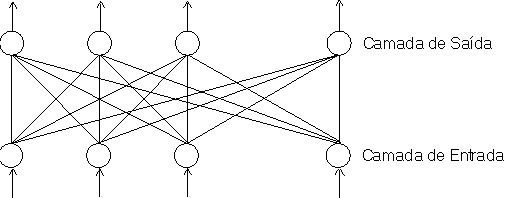
\includegraphics[width=90mm, height=30mm]{Figuras/Neural/Rosenblatt.png}\\
\tiny Fonte: http://www.din.uem.br/ia/neurais/neural. Acessado em: 01/10/2016
\end{figure}


Dando continuidade e indo mais além dos trabalhos de Rosenblatt e seus colaboradores, Widrow desenvolveu, em conjunto com alguns 
alunos, o Adaline, um tipo de processamento de redes neurais dotado de uma potente lei de aprendizado, em uso ainda nos dias atuais, 
que pode ser representado pela figura abaixo:

\begin{figure}[!ht]
\centering
\caption{Rede ADALINE e MADALINE}
\vspace{1mm}
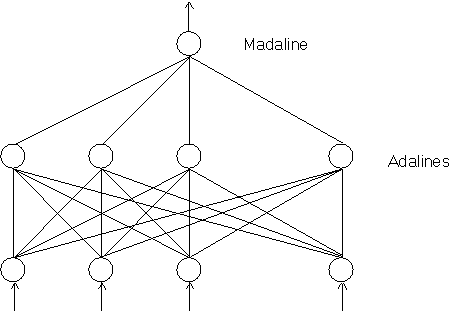
\includegraphics[width=85mm, height=40mm]{Figuras/Neural/Adaline.png}\\
\tiny Fonte: http://www.din.uem.br/ia/neurais/neural. Acessado em: 01/10/2016
\end{figure}

\pagebreak

Muitos estudos foram realizados nas décadas seguintes, mas o que marcou esse período foram as elucubrações sobre o 
desenvolvimento de máquinas tão potentes quanto o cérebro humano, muito mais do que a publicação de pesquisas realmente 
contundentes na área.

A partir dos anos 80, a pesquisa em neurocomputação deu outro grande salto qualitativo e em 1987 teve lugar, em São Francisco a 
primeira conferência de redes neurais nos tempos modernos: a IEEE International Conference on Neural Networks, sendo também formada 
a International Conference on Neural Networks Society (INNS). 
Em 1989 foi fundado o INNS Journal, e em 1990 o Neural Computation e IEEE Transations on Neural Networks.

\subsection{Definições e funcionamento de uma Rede Neural Artificial}

São várias as definições que podem ser encontradas sobre o que vem a ser uma Rede Neural Artificial (RNA) \cite{Castanheira}, em função da complexidade de tal Rede. 
Do ponto de vista computacional, uma RNA configura-se como uma técnica para solucionar problemas de Inteligência Artificial (IA) que estabelece um modelo matemático 
baseado em funções de um modelo neural biológico simplificado, com capacidade de aprendizado, generalização, associação e abstração.

Uma grande rede neural artificial pode ter centenas ou milhares de unidades de processamento, enquanto que o cérebro de um mamífero pode ter muitos bilhões de neurônios. 
Uma Rede Neural Artificial (RNA) é um sistema que de neurônios que estabelecem conexões sinápticas, que possuem neurônios de entrada, que recebem os estímulos provenientes 
do meio exterior, os neurônios internos ou hidden (neurônios ocultos) e os neurônios de saída, que se comunicam com o mundo externo \cite{Tatibana}.

Cabe destacar que, de acordo com esse modelo, os neurônios internos têm considerável importância nesse processo, uma vez que são responsáveis pela resolução de problemas linearmente inseparáveis. 
O comportamento inteligente de uma Rede Neural Artificial vem das interações entre as unidades de processamento da rede.

Os neurônios, nessas redes são conhecidos como Perceptrons. O arranjo em camadas desses perceptrons é chamado \textit{Multilayer Perceptron}.
O \textit{multilayer perceptron} é responsável pela resolução de problemas mais complexos que não seriam passíveis de resolução pelo modelo 
de neurônio básico. Para aprender os perceptrons tem que estar dispostos em camadas, um único perceptron pode realizar algumas operações do 
tipo XOR, contudo seria incapaz de aprendê-la.

A figura a seguir apresenta o arranjo dos perceptrons em camadas, conforme discutido anteriormente.
\pagebreak

\begin{figure}[!ht]
\centering
\caption{Um arranjo de Perceptrons em camadas}
\vspace{1mm}
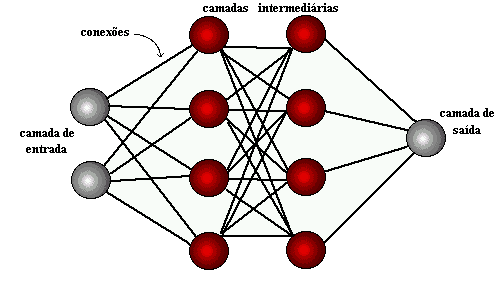
\includegraphics[width=90mm, height=50mm]{Figuras/Neural/camdasIntermediarias.png}\\
\tiny Fonte: http://www.din.uem.br/ia/neurais/neural. Acessado em: 01/10/2016
\end{figure}

São três as camadas usualmente identificadas em uma rede de perceptrons:
\begin{itemize}
 \item Camada de entrada: nessa camada apresenta-se os padrões à rede;
 \item Camadas Intermediárias (ocultas): aqui é realizada a maior parte do processamento por conexões ponderadas. São consideradas como as camadas 
 extratoras de características;
 \item Camada de saída: responsável pela conclusão e apresentação do resultado.
\end{itemize}

O comportamento inteligente de uma Rede Neural Artificial vem das múltiplas interações existentes entre as unidades de processamento dessa rede. 
As unidades de processamento são conectadas por canais de comunicação, associados a determinado peso, como mostra a figura a seguir, proposta por McCulloch e Pitts (1943)

\begin{figure}[!ht]
\centering
\caption{Perceptron de McCulloch e Pitts}
\vspace{1mm}
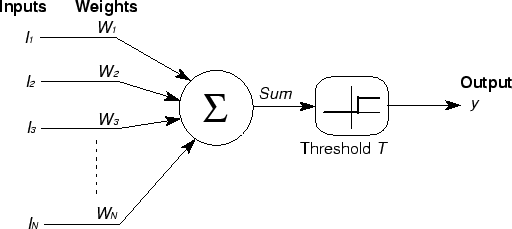
\includegraphics[width=90mm, height=40mm]{Figuras/Neural/Perceptron.png}\\
\tiny Fonte: http://www.din.uem.br/ia/neurais/neural. Acessado em: 01/10/2016
\end{figure}

Esses canais são os  \textit{inputs}, $ I_{1}, I_{2}, I_{3},...,I_{n}$, e cada um tem um peso associado, que serão calibrados de acordo 
com a aproximação do resultado esperado pela rede neural, produzido na saída (fase de ``forward''). 
Essa aproximação é conhecida como erro ou erro padrão. Esse erro será propagado de volta à entrada, retroalimentando a rede neural (fase de ``backward''), 
caso o modelo de rede de aproximação seja o ``backpropagation''. Dessa forma a rede neural se aproxima cada vez mais do resultado que foi previamente estimado; fase de treinamento.
Uma vez que o erro tornar-se infinitamente pequeno dizemos que a rede neural ``não aprende mais'' há uma degradação do sistema, o ``overfitting''.


Da figura acima podemos extrair duas coisas:
\begin{itemize}
 \item A função calculada \textit{y} é uma função \textbf{discriminativa} (classificação) com $y=0$ e $y=1$.
    \begin{itemize}
     \item $net = x_1w_1 + x_2w_2 + ... + x_iw_i + x_dw_d = \sum x_i.w_i = W.X = W^T X$
     \item $onde\ w = \{+1, -1\}$
     \item $saida = y = f(net)$
     \item $f(net)= \left \{ \begin{matrix} 1, & se\ net \ge \mu \\ 0, & se\ net < \mu \end{matrix} \right. $
    \end{itemize}
\vspace{1mm}
 \item Fronteira de Decisão:
    \begin{itemize}
     \item [--] Determina o ponto que separa os dados que vêm de -$\infty$ e +$\infty$
     \item [--] Argumento de $f(net)$ é igual a zero: $\sum w_ix_i - \mu \Rightarrow w.x = 0$
    \end{itemize}
\end{itemize}

\vspace{2mm}

O modelo McCulloch e Pitts (1943) leva em conta cinco hipóteses fundamentais, a saber:

\begin{enumerate}
 \item A atividade de um neurônio é binária. Isso quer dizer que os neurônios respondem a valores \textbf{verdadeiro} ou \textbf{falso} ou 0 ou 1;
 \item As RNA são formadas por linhas direcionadas, que são inspiradas em sinapses, e que ligam os neurônios. Tais linhas podem ser positivas (excitatórias) ou negativas (inibitórias);
 \item Os neurônios, numa RNA, têm um limiar fixo, nomeado como L. Isso posto, o processo só é disparado se a entrada for igual ou maior que esse limiar;
 \item Uma única sinapse inibitória evita, por completo, o disparo do neurônio, ainda que venham, ao mesmo tempo, várias sinapses excitatórias;
 \item A quinta e última hipótese propõe que cada sinal leva determinada unidade de tempo para ``passear'' de um neurônio a outro.
\end{enumerate}

Uma rede neural passa por um processo de treinamento, estabelecido a partir de casos reais, que a faz adquirir, a partir de então, a sistemática que é necessária para executar o processo desejado satisfatoriamente. Isso faz com que as RNA tenham uma característica diferente da computação programada, que exige um conjunto de regras pré-fixadas e algoritmos. 
A Rede Neural, por sua vez, extrai regras básicas a partir de dados reais, ou seja, aprendem através de exemplos.
Uma vez ``treinada'' os pesos estão calibrados para solucionar a classe de problemas para o qual foi desenhada. Essa rede neural portanto pode ser 
considerado um aproximador de funções, uma vez dada uma série de ``inputs'' ela poderá produzir um ``output'' baseada nas funções de internas.

\subsection{Aplicações e Tipos de Redes Neurais}

São várias as aplicações das redes neurais. Elas podem ser utilizadas para reconhecimento e classificação de padrões;
processamento de sinais e de imagens; identificação e controle de sistemas; predição, dentre outras funções. 
No caso específico desse estudo, nosso interesse está centrado, fundamentalmente, na predição.

Para o desenvolvimento de uma rede neural algumas importantes fases precisam ser consideradas. 
Em primeiro lugar, é necessário um estudo detalhado do problema, para que possam ser feitas as escolhas adequadas à sua resolução. 
Em seguida, passa-se à fase de desenvolvimento do modelo neural, a partir de neurônios biológicos, e das estruturas e conexões sinápticas. 
A etapa seguinte implica na escolha de um algoritmo de aprendizado de regras, com ajuste de pesos ou forças de conexões intermodais, e de um conjunto de treinamento. 
Passa-se, então, à fase de treinamento, propriamente dita, aos testes e, por fim, utilização da rede neural.

Uma vez que existem distintas possibilidades de aplicação e desenvolvimento de uma RNA, existem, igualmente, diversas maneiras de 
classificá-las \cite{AAP}. Trataremos de algumas dessas nesse tópico.

\begin{itemize}
 \item [(a)] Quanto à sua arquitetura: estática, dinâmica ou fuzzy; de única camada/camadas simples ou de múltiplas camadas.
	   Exemplos de RNA de uma (i) ou múltiplas (ii) camadas:
	    \begin{enumerate}
	      \item [(i)] São exemplos de redes Percepton e Adaline
	      \begin{figure}[!ht]
		\centering
		\caption{Perceptron e Adaline}
		\vspace{1mm}
		  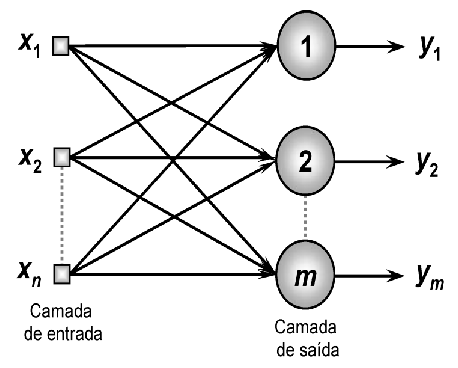
\includegraphics[width=85mm, height=50mm]{Figuras/Neural/pecepAdalin.png}\\
		\tiny Fonte: http://www.dkriesel.com. Acessado em: 10/10/2016
	      \end{figure}
	 %+++++++++++++++++++++++++++++++++++++++++++++++++++++++++++++++++++++++++++++++++++++++++++++++++++   
	      \item [(ii)] São exemplo dessas redes as de Perceptron multicamadas (PMC/MLP) e redes de base radial (RBF)
	      \begin{figure}[!ht]
		\centering
		\caption{Perceptron Multicamadas}
		\vspace{1mm}
		  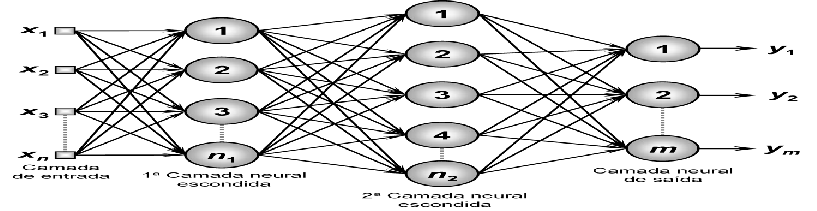
\includegraphics[width=110mm, height=70mm]{Figuras/Neural/MultiCamadas.png}\\
		\tiny Fonte: http://www.dkriesel.com. Acessado em: 10/10/2016
	      \end{figure}

	      Alguns autores ainda fazem referência às redes recorrentes ou realimentadas (iii), 
	      como a rede de Hopfield e a Perceptron multicamadas \cite{Kriesel2007NeuralNetworks}. 
	      Tais redes, segundo esses autores, são ideais para processamento dinâmico, como previsão de 
	      séries temporais, controle de processos, etc.
	      Referem também a existência das redes com estrutura reticulada (iv), como a rede de Kohone.
	%+++++++++++++++++++++++++++++++++++++++++++++++++++++++++++++++++++++++++++++++++++++++++++++++++++
	      \item [(iii)] Exemplo de rede recorrente ou realimentada: ``backpropagation''
	      \begin{figure}[!ht]
		\centering
		\caption{Perceptron com Realimentação}
		\vspace{1mm}
		  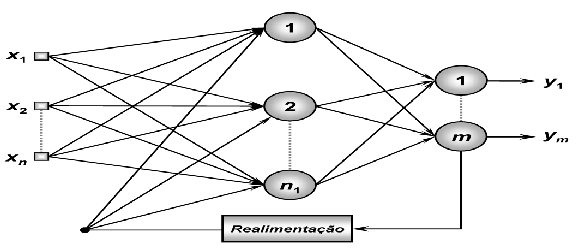
\includegraphics[width=100mm, height=65mm]{Figuras/Neural/Recorrentes.png}\\
		\tiny Fonte: http://www.dkriesel.com. Acessado em: 10/10/2016
	      \end{figure}  
	 
	 %+++++++++++++++++++++++++++++++++++++++++++++++++++++++++++++++++++++++++++++++++++++++++++++++++++   
	      \item [(iv)] Exemplo de redes de estrutura reticulada
	      \begin{figure}[!ht]
		\centering
		\caption{Rede Kohone}
		\vspace{1mm}
		  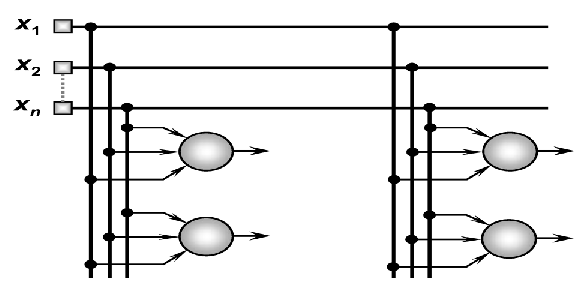
\includegraphics[width=100mm, height=65mm]{Figuras/Neural/Kohone.png}\\
		\tiny Fonte: http://www.dkriesel.com. Acessado em: 10/10/2016
	      \end{figure}
	
	\end{enumerate}

\pagebreak
	
  \item [(b)] Quanto às conexões, os tipos de RNA são: no sentido de ida; no sentido de ida e volta; 
	      lateralmente conectadas; topologicamente ordenadas; híbridas.
  
  \item [(c)] Quanto à aplicação: reconhecimento de padrões e classificação; processamento de imagem e visão; 
	      identificação de sistema e controle; processamento de sinais.
\end{itemize}


\subsection{Aprendizado em Redes Neurais}

O aprendizado caracteriza-se pela capacidade que a RNA tem de resolver uma determinada classe de problemas para os quais foi destinado 
seu desenvolvimento. 
Nesse processo, é proposto um algoritmo de aprendizado, que se caracteriza como um conjunto de regras bem delineadas que permitirão a 
resolução do problema. 

O aprendizado das RNA resulta da fase de treinamento, através de um processo iterativo de ajuste dos pesos. 
O conhecimento é armazenado nas sinapses, ou seja, nos pesos que são atribuídos às conexões que existem entre os neurônios da rede.

\begin{itemize}
 \item Por independência de quem aprende: o aprendizado pode ser por memorização, por contato, por exemplos, por analogias, por 
	exploração, por descoberta, sobretudo por uma mistura entre os últimos três \cite{Barreto2002}.
 \item Por retroação do mundo: quando há uma realimentação específica vinda do mundo exterior, podendo ser supervisionado ou 
	não-supervisionado. 
\end{itemize}

O treinamento supervisionado tem sido o mais comumente utilizado em redes neurais \cite{Barreto2002}. 
Em linhas gerais, como o nome indica, no treinamento supervisionado há um agente externo que indica explicitamente à rede um 
comportamento bom ou ruim, com base no padrão de entrada. Os valores iniciais dos pesos são aleatórios, e o ajuste se dá a partir do 
algoritmo de aprendizado, na próxima interação ou ciclo seguinte. São apresentados sinais de entrada e de saída à rede, e os ajustes 
vão sendo feitos paulatinamente. O treinamento pode levar um período considerável de tempo, em função dos ajustes que vão sendo 
realizados. O treinamento é concluído quando a rede neural atinge um determinado patamar de desempenho, tendo alcançado a precisão 
estatística esperada. 
Não havendo mais necessidade de treinamento, “congela-se” os pesos, para sua aplicação. 

O aprendizado não supervisionado, por sua vez, não depende de um agente externo, pois funciona de forma autorregulatória, apresentando 
mecanismos que analisam as regularidades ou tendências dos padrões de entrada, possuindo a capacidade de se adaptar automaticamente às 
necessidades da rede. 

O aprendizado de uma rede se dá em um determinado tempo e a partir de determinado padrão. 
A velocidade de aprendizado depende de variáveis que precisam ser consideradas como, por exemplo, a complexidade da rede proposta, 
a quantidade de camadas que ela possui, a arquitetura adotada, o algoritmo que foi utilizado, a precisão esperada. 
É preciso que se esteja atento a todos esses elementos, uma vez que dependendo de como essas variáveis forem consideradas, 
o treinamento pode se estender por um período bastante longo e, nem sempre apresentando um resultado satisfatório.

Quanto aos algoritmos de aprendizagem, são muitos os que podem ser utilizados, mas boa parte deles são variações do princípio de Hebb, 
que é a regra mais utilizada \cite{Barreto2002}. A descrição dessa regra foi apresentada pelo seu propositor, Donald Hebb, em 1949. 
A ideia básica dessa regra é a de que quando um neurônio recebe um entrada a partir de outro neurônio, isso significa que ambos 
estão ativos e que os pesos entre os neurônios precisam ser excitados.

Uma segunda lei utilizada é a de Hopfield. Ela se inspira no princípio de Hebb, mas acrescenta a ideia de definição da magnitude da 
excitação ou inibição. Uma terceira regra, que é a mais comumente utilizada hoje em dia, é a regra Delta de Widrow. 
Essa regra propõe a alteração dos pesos sinápticos, minimizando o erro quadrático da rede, reduzindo a diferença entre o valor de saída 
desejado e o atual valor de saída da unidade de processamento. 
Assim, o erro da saída é transformado pela derivação da função de transferência e utilizado pra regular os pesos de entrada da camada 
prévia da rede, realizando assim um processo de retropropagação dos erros. 
Para a utilização desse tipo de regra deve-se observar que o conjunto dos dados de entrada esteja organizado de forma aleatória. 

Há ainda a lei de aprendizado de Teuvo Kohonen, que foi inspirada em sistemas biológicos, em que há uma competição entre os elementos 
para aprender, ou atualizar e ajustar seus pesos. A unidade de processamento mais apta será aquela que possuir o melhor sinal de 
saída e terá a capacidade de inibir os ajustes sinápticos de seus concorrentes e excitar seus vizinhos, de maneira que apenas essa 
unidade e seus vizinhos poderão realizar o ajuste dos pesos.

\subsection{Retropropagação e o Erro médio quadrático}



\section{Medida de desempenho e qualidade aplicadas à mineração}

Quando são desenvolvidos sistemas de predição e análise de diagnóstico, avalia-se o desempenho e a qualidade dos resultados encontrados.
Um método gráfico eficiente para detecção e avaliação da qualidade de sinais, conhecido como \textit{Receiver Operating Characteristic} -- ROC, ou curva ROC \cite{ROC},
foi criado e desenvolvido na década de 50 do século passado, para avaliar a qualidade da transmissão de sinais em um canal com ruído.
Recentemente a curva ROC tem sido adotada em Mineração de dados e Aprendizagem de Máquina \cite{MD_AM}, em sistemas de suporte à decisão na medicina, para analisar a qualidade da detecção 
de um determinado teste bioquímico, na psicologia para detecção de estímulos \cite{Discriminativo} em pacientes, e na radiologia para classificação de imagens.

Essas métricas são amplamente utilizadas na classificação binária de resultados contínuos. Para isso ser construído utiliza-se a Matriz de Contingência que classifica as probabilidades como:
verdadeiro positivo, falso positivo, falso negativo e verdadeiro negativo, respectivamente \textit{True Positive -- TP, False Positive -- FP, False Negative -- FN e True Negative -- TN },
também conhecida como matriz de confusão, descrita na tabela a seguir:

%tabela 5
\begin{table}[ht]
\centering
\caption{Matriz de Confusão}
\vspace{1mm}
\begin{tabular}{l|c|c}
\hline
\textbf{} & \textbf{Predito} & \textbf{}\\
\hline
\textbf{Real}  & TP   FN & Positive -- POS\\
\textbf{Real}  & FP   TN & Negative -- NEG\\
\hline
   ---         & PP   PN &    ---         \\
\end{tabular}
\tiny Fonte: \cite{Bradley1997}
\end{table}

A matriz da Tabela 2.3 sintetiza a matriz da Tabela 2.4, portanto as duas tabelas são equivalentes.

%tabela 6
\begin{table}[ht]
\centering
\caption{Matriz modelo de Confusão}
\vspace{1mm}
\begin{tabular}{l|c|c}
\hline
\textbf{}           & \textbf{Y}     \textbf{$\bar{Y}$}   & \textbf{}\\
\hline
\textbf{X}          & P(X,Y)         P(X,$\bar{Y}$)       & Positive -- POS\\
\textbf{$\bar{X}$}  & P($\bar{X}$,Y) P($\bar{X},\bar{Y}$) & Negative -- NEG\\
\hline
   ---              & P(Y)           P($\bar{Y}$)         &     ---        \\
\end{tabular}
\tiny Fonte: \cite{Bradley1997}
\end{table}


De acordo com as probabilidades condicionais temos:

\begin{equation}
 P(X,Y) = P(X|Y).P(Y) = P(Y|X).P(X)
\end{equation}

Então, a taxa de verdadeiros positivos será $P(Y|X)$ e a probabilidade de falsos alarmes ou taxa de falsos positivos será $P(Y,\bar{Y})$, a barra sobrescrita em $\bar{X}$
(ou $\bar{Y}$) representa negação. \\
A curva ROC será construída cruzando-se a taxa dos verdadeiros positivos (tpr = P(Y|X)) com a taxa dos falsos positivos (fpr = P(Y,$\bar{X}$)).

\pagebreak

\subsection{Coeficiente de Gini para dados socio-econômicos}

\pagebreak



\section{Redes sociais}

As redes sociais são um arcabouço de informações sobre todo tipo de assunto vivenciado no cotidiano das pessoas, inclusive situações que dizem respeito ao nosso ambiente de pesquisa.
O cenário abaixo, encontrado numa rede social, exemplifica a sequência de informações retiradas do Twitter, um microblog onde os usuários escrevem num pequeno espaço (cerca de 140 caracteres), 
os mais diversos assuntos, e os usuários conectam por uma multiplicidade de dispositivos: computadores, tablets e celulares, formando uma grande rede social mundial. 
A ideia inicial do Twitter, segundo seus fundadores, era que essa rede se comportasse como um ``SMS da Internet'' \cite{Twitter2015}. 
As informações são enviadas aos usuários, conhecidas como twittes, em tempo real e também enviadas aos usuários seguidores que tenham assinado para recebê-las.

"Em 2010 empresas e usuários armazenaram mais de 13 exabytes de novos dados" \cite{bigdataQualquerUm}.

%tabela 5
\begin{table}[!ht]
\centering
\caption{Volume de dados no mundo}
\vspace{1mm}
\begin{tabular}{l|c|c|c}
\hline
\textbf{Ano} & \textbf{Qtd} & \textbf{Unidade} & \textbf{Múltiplo}\\
\hline
2000 & 800 & terabytes – TB & $10^{12}$\\
2006 & 160 & petabytes – PB & $10^{15}$\\
2009 & 500 & exabytes – EB & $10^{18}$ \\
2012 & 2,7 & zettabytes – ZB & $10^{21}$\\
2020 & 35 & yottabytes – YB & $10^{24}$\\
\end{tabular}
\end{table}

------------------
Artigo ``Library \& Information Science Research''

Introdução
Usuários de redes sociais gastam uma quantidade de tempo crescente a cada ano. 
Estes partilham informações, conhecimento e atividade de lazer (i.e. jogos).
Neste paper descobriu-se que mais de 70\% dos adultos que estão on-line utilizam redes sociais, 20\% desses utilizam o Twitter, 46\% visitaram diariamente e desses 29\% o fizeram mais de uma vez ao dia (Duggan \& Smith, 2013).
Another Pew num relatórios mostrou que o Twitter está ranqueado entre as três maiores plataformas de mídias sociais (após o Facebook e o Youtube). Nos EUA 8\% dos adultos entre 18 e 29 anos o Twitter está ranqueado a frente do Facebook e Youtube, com 45\% dos adultos de outras idades nos EUA. O principal item de consumo são: notícias (Mitchell \& Page, 2013). Num dia normal o Twitter possui mais de 230 milhões de usuários que produzem cerca de 500 milhões de tweets (postagem tipo microblog) (Twitter, 2014)


Revisão da Literatura
Blogs são sistemas de compartilhamento de informações baseados na Web, com conteúdo postados  em ordem cronologicamente (Hering, Scheid, Bonus \& Wright, 2004).
Twitter é um sistema de microblog que está restrito ao tamanho do conteúdo entrado (postado) em 140 caracteres. Adicionalmente o Twitter  provê a capacidade de usuários poderem seguir outros usuários, partilhar com eles conteúdos e conversação (Twitter, 2014).
Relevantes literaturas examinam conteúdos de tweets de amostras de usuários do Twitter. Heneycutt e Hering (2009) identificaram 11 catagorias de conteúdo dos tweets: sobre destinatários, anúncio/propaganda, encorajamento “exhort” (talvez auto-ajuda), informações para outros, informações para si próprio, meta comentários, uso de mídia, expressar opinião, outras experiências, auto experiência, e solicitação de informações. 
Para Naaman, Boase e Lai (2010) a tipologia de conteúdo inclui-se em oito categorias: Informações compartilhadas, auto promoção, opinião/queixas, declarações e pensamentos aleatórios, eu agora, (me now), perguntas aos seguidores, manutenção de presença, e piadas. 
André, Berstein e Luther (2012) adaptaram a tipologia de Naaman et al. para avaliar o relacionamento entre categorias de tweet e o valor para os usuários numa amostra geral de usuários do Twitter e tweets. A tipologia adaptada incluiu categorias de seguidos: perguntas para os seguidores, informações partilhadas, auto promoção, ideias aleatórias, opinião, eu agora (me now), conversação e manutenção de presença.
Na Cientometria e Bibliometria contar citações são frequentemente usados para avaliar o impacto de uma publicação; escolar, centro de pesquisas ou instituições (i.e. Adkins \& Budd, 2006; Cronin \& Overfelt, 1994; Cunningham \& Dillon, 1997; Lee, 2003). Posteriormente, pesquisadores examinaram a relação entre características dos autores e grupo de autores e o impacto da produtividade deles, foi medido o número de publicações produzidas e o número de citações recebidas (Haslam et al., 2008;  Hinnant el al., 2012; Stivilia et al., 2011).
Na Web o número de citações (i.e. links de URL) e a estrutura dos links são usadas pelas “engenhocas de pesquisas”(poderia ser traduzido como moteres de busca, ex: o google) para identificar a importância ou autoridade de websites (Brin \& Page, 1998), similarmente o número de seguidores, menções a usuários e retweets fora usados para avaliar a influência ou impacto dos usuários do Twitter e tweets. 
No Twitter, a conexão entre os usuários da rede social são estabelecidas pelos seguidores e os seguidos pelos links . Indo além, a habilidade do seguidor para retweetar os usuários seguido serve de principal mecanismo de espalhar informações através dessas redes. 
Cha, Haddadi e Benevenuto (2010) avaliaram a influência dos usuários no Twitter analisando o número de retweets, menções e seguidores. Através disso, no geral eles encontraram uma correlação positiva entre o número de seguidores e o número de retweets pelo top 10 (do Twitter) e o primeiro percentil dos mais conectados, baseados no grau do link (i.e. número de seguidores), o número de seguidores não está relacionado com o número de retweets ou número de menções. André et al. (2012) usou a abordagem “crowdsourcing” para identificar os tipos de tweets dos usuário do Twitter que gostam e não gostam. Eles encontraram que os usuários preferem perguntar aos seguidores, partilhar informações e auto promoção. Os usuários não tem preferido os tweets categorizados como: manutenção de presença, conversações e atualizações do “status” corrente do usuário.
Suh, Hong e Chi (2010) encontraram uma correlação positiva entre a presente URL de um tweet e a probabilidade de um retweet. Adicionalmente eles encontraram relações positivas entre o número de usuários seguidos e seguido pela probabilidade de retweet, embora com tamanho de efeito muito pequeno.

Artigo “A Text Mining Analysis of Academic Libraries Tweets”


Introdução
Aplicações de mídia sociais tem cada vez mais sido adotadas pelo marketing das bibliotecas com recursos e serviços (Collins \& Quan-Haase, 2014) para incrementar os relacionamentos entre seus  clientes. Ele permite “compartilhar informações e conhecimentos, incrementar serviços e promoções, interação com estudantes usuários das bibliotecas, a um custo mínimo” (Chue \& Due, 2013, p. 72). Bibliotecas acadêmicas estão adotando as mídias sociais e essa prática tem mudado dramaticamente como elas interagiam com os usuários (Del Bosque, Leif e Skaf, 2012). Por exemplo o Twitter pode criar um relacionamento forte com os clientes (Cavanagh, 2015) isto é “usado” como alternativa para um canal de comunicação e bem utilidade social para formar uma conexão personalizado com os usuários (Boaten \& Quan, 2014).
Nessa veia as bibliotecas academicas tem vindo proativamente responder às mudanças envolvendo tecnologia (Shulman, Yep e Tomé, 2015)….

-------------------------------

A seguir pode-se verificar uma sequência de twittes da Polícia Rodoviária Federal de Santa Catarina:

\begin{figure}[ht]
\subfigure{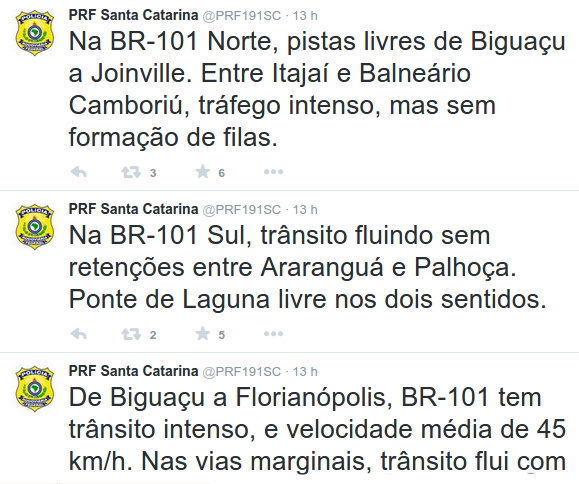
\includegraphics[width=60mm, height=48mm]{Figuras/BigData/twittePRF.png}}
\quad \quad \quad \quad
\subfigure{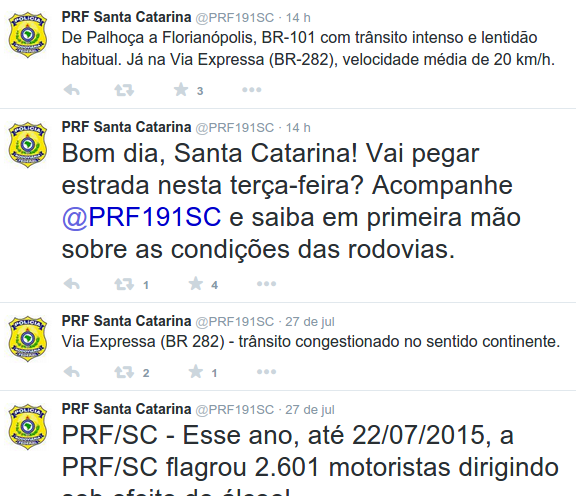
\includegraphics[width=60mm, height=48mm]{Figuras/BigData/twittePRF2.png}}
\end{figure}

A Polícia Rodoviária Federal de Santa Catarina, disponibilizou às 13h através do canal @PRF191SC, informações relevantes sobre o trânsito naquela localidade, 
num espaço temporal variado, por exemplo: entre Itajaí e Balneário Camboriú o transito está intenso. Isso sugere que a frota de caminhões deva ter uma
rota alternativa caso a situação persista por muito tempo. No primeiro twitte da segunda coluna, é informado em Via Expressa (BR 282) que o trânsito está lento com 
velocidade de 20km/h (praticamente congestionado). Essa informação sugere que deve ser pensada uma rota alternativa, caso o congestionamento persista por muito tempo.

Outra rede social conhecida pelos condutores de veículos é o Waze. O Waze é um aplicativo de navegação para o trânsito, funciona em aparelhos celulares e tablets. 
Os utilizadores desse aplicativo são conhecidos como wazers e compartilham informações sobre o trânsito, em tempo real. Toda via, as informações somente estão disponíveis 
no momento em que são postadas pelos utilizadores, por um período de tempo pequeno. Caso não haja usuários trafegando pelas vias ou caso os mesmos não tenham disponibilidade 
em postar informações, não há o que se compartilhar.
Outro problema levantado com o waze é que, caso não haja conexão à Internet não há como acessar os dados dos 'wazers', para navegação.

Além dos dados que chegam ao \textit{Big Data} através das redes sociais, as grandes cidades têm disponíveis câmeras de monitoramento do trânsito nos semáforos ou próximas a eles; 
algumas com cobertura por canais de televisão bem como câmaras de segurança próximos às rodovias, coletando informações em tempo real. 
Os dados desses dispositivos são gravados, sendo conhecidos como \textit{stream} de dados. 
Esses \textit{streams} podem ser disponibilizados na Internet, em sítios eletrônicos especialmente construídos para isso, como o http://vejoaovivo.com.br dentre outros.

Os dados disponibilizados pelos diversos meios de comunicação não estão em formato que possam ser utilizados imediatamente, precisando antes serem processados. 
Tais dados não processados são conhecidos como ``dados frios''. O processo de tratar as informações, retirando-lhes o ``lixo'' e transformando dados ``frios'' em dados 
``quentes'', é um processo que tem um custo temporal elevado, devido ao volume dos dados.



\pagebreak
\subsection{Data Mining - Text Data Mining}\label{arte:palavraChave:DataMiningBigData}

Minerar dados em texto nas redes sociais não é uma tarefa atômica, devendo ser divida em várias etapas, com processos específicos em cada uma delas, como descrito anteriormente. 
Extrair conhecimento dos dados não processados não faz sentido, tratá-los apenas ``per si'' exige muito trabalho de IA, como Mineração de dados em textos. 
A Mineração em textos é inspirada em técnicas de ``Machine Learning'' \cite{Aranha2006}. 
Contudo analisar textos é basicamente entender o significado do texto, baseado em regras de associação lógica.
O mapa mental a seguir mostra um modelo de análise de texto feito por seres humanos.

\begin{figure}[htpb]
\centering
\caption{Mapa mental da Mineração em textos}
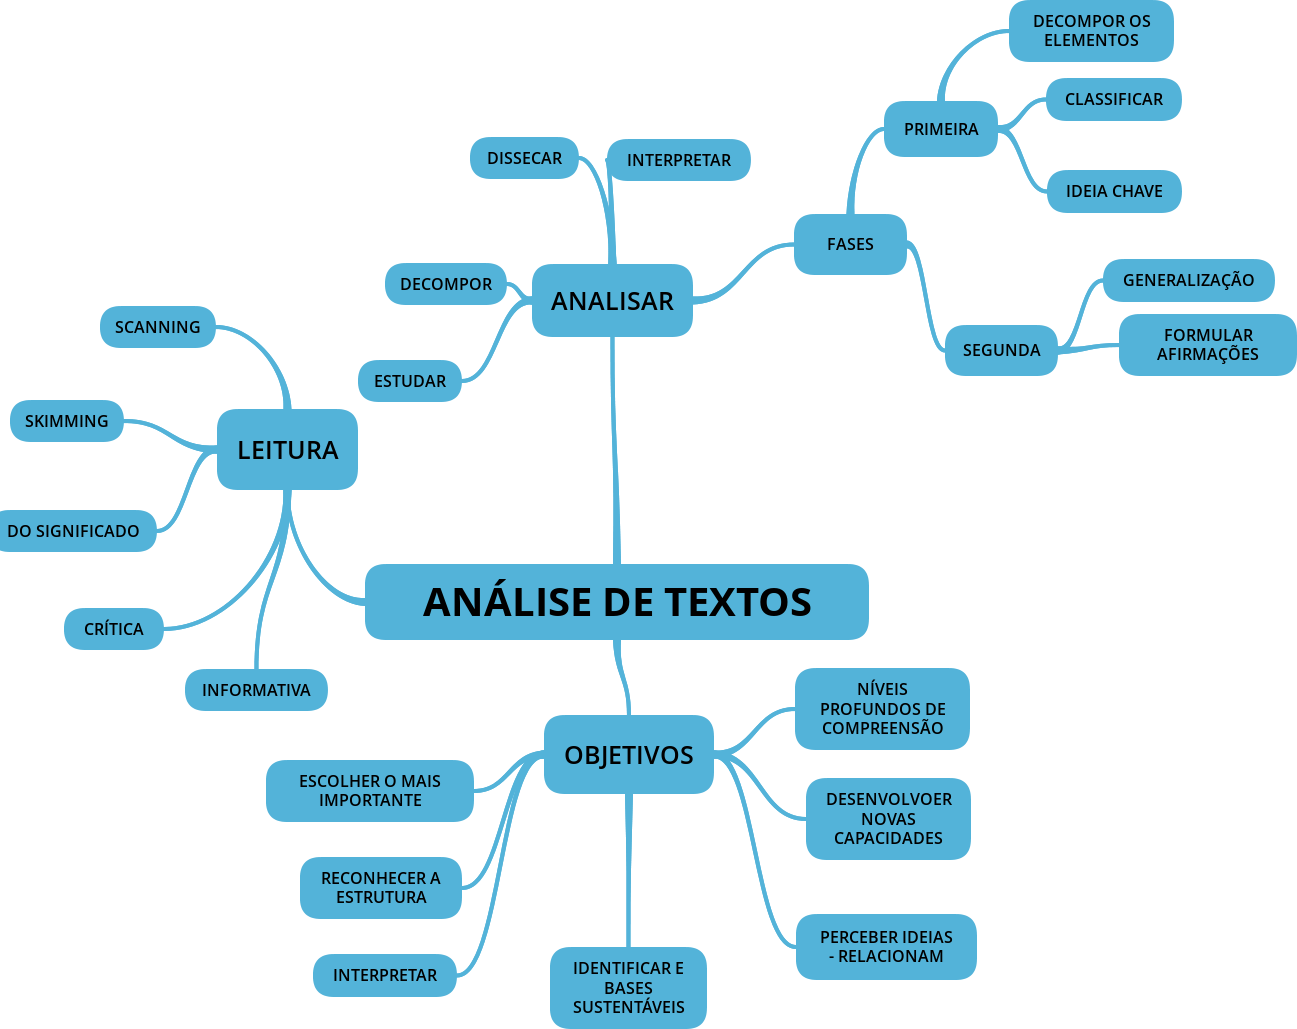
\includegraphics[width=120mm, height=60mm]{Figuras/BigData/Analise_Textos.png}
\end{figure}

\pagebreak

\section{Cibernética: aspectos introdutórios}

Cibernética é um termo proveniente do grego que significa timoneiro, piloto, ou ``quem está no comando do navio''.
Atribui-se à Norbert Wiener (1894 -- 1963), matemático e professor do \textit{Massachusetts Institute of Technology} (MIT) o termo Cibernética, quando publicou o livro 
\textit{Cybernetics, or Control and Communication in the Animal and the Machine} (Wiener, 1948).
``A Cibernética é a ciência da comunicação e do controle nos animais e a nas máquina, salientando que o \textit{ser vivo é uma máquina entre 
cujas funções, uma é a de montar a própria máquina}. E isto porque \textit{os organismos só atuam graças à aquisição, ao uso, à conservação 
e à transmissão da informação}''  \cite{Maltez1991}.

Wiener propôs que informação é tão importante quanto a energia e a matéria \cite{Salles2007}. Essa informação poderia ser utilizada para controlar um sistema baseado em 
comportamento; biológico ou mecânico. Esse comportamento, quando responde à informação por meio de realimentação, é chamado de teleológico ou controlado por meio de 
realimentação, tendo em vistas a atingir um objetivo, um propósito.




